\documentclass[german,version-2019-11]{uzl-thesis}
\UzLThesisSetup{
  Logo-Dateiname        = {uzl-thesis-logo-itcs.pdf},
  Verfasst              = {am}{Institut für Theoretische Informatik},
  %
  % The titles:
  %
  Titel auf Deutsch     = {
    Algorithmen für das Moving-Target-Travelling Salesman Problem
  }, 
  Titel auf Englisch    = {
    Algorithms for the Moving-Target-Travelling Salesman Problem
  },
  Autor                 = {Felix Greuling},
  Betreuerin            = {Prof. Dr. Maciej Liskiewicz},
  Bachelorarbeit,
  Studiengang           = {Informatik},
  Datum                 = {29. Dezember 2019},
  Abstract              = {
    \textcolor{red}{TODO}
    
  },
  Zusammenfassung       = {
    \textcolor{red}{TODO}  
  },
  %Acknowledgements      = {}, 
  % Alphabetische Bibliographie
  % Alternatively:
  Numerische Bibliographie
}

% \UzLStyle{pagella basic design}
% \UzLStyle{pagella centered design}
% \UzLStyle{pagella contrast design}
% \UzLStyle{alegrya basic design}
% \UzLStyle{alegrya scholary design}
% \UzLStyle{alegrya stylish design}
\UzLStyle{alegrya modern design}
% \UzLStyle{thesis black and white structure}

% Now, include the package you need here using \usepackage. 
% \usepackage{graphicx,float,wrapfig}
\usepackage{mathtools}
\usepackage{algorithm}
\usepackage{algpseudocode}

%tikz
\tikzstyle{gray}  = [thick, color=gray, circle, draw]
\tikzstyle{red}   = [thick, color=red, circle, draw]
\tikzstyle{blue}  = [thick, color=blue, circle, draw]
\tikzstyle{green} = [thick, color=green, circle, draw]

\newtheorem{lem}{Lemma}

% begin of the document
\begin{document}
% \chapter{Introduction}
\chapter{Einleitung}

Das Travelling-Salesman-Problem (TSP) ist ein in der Informatik weit verbreitetes und seit der Formulierung im Jahre 1930 als mathematisches Problem ein langjährig erforschtes Optimierungsproblem aus der Kombinatorik. Dies hat eine besonders hohe Relevanz für alltägliche Probleme, da diese auf das TSP reduziert werden können. Gesucht ist dabei eine Reihenfolge an Wegen, welche die Ziele miteinander verbinden, sodass 
die Tourzeit minimal ist. In dieser Tour muss jedes Ziel über die Wege besucht werden. Sofern die Tour eine Rundtour ist, wird jene auch im Startpunkt beendet. Betrachten dafür eine Menge an Städten. Diese sollen allesamt von einem FlixBus als Zwischenstop genutzt werden, da an diesem Reisende aus- und einsteigen wollen. Am Ende der Tour soll der FlixBus zum Auftanken wieder zu seinem Ausgangspukt zurückgelangen. Um die Benzinkosten gering zu halten, wird also die kürzeste Abfolge an Städten gesucht. Dabei sollte man beachten, dass mehrere optimale Touren möglich sind. Für TSP gibt es gerade heutzutage diverse Anwendungsgebiete. Wir leben in einem Zeitalter, in welchem autonome Systeme zunehmend eine große Rolle spielen. Früher oder später übernehmen autonome Fahrzeuge die Verantwortung auf unseren Straßen \cite{minx2015autonomes}. Der Vorreiter für diesen Markt ist die Firma Tesla. Die Fahrzeuge besitzen bereits die Software zum selbstständigen Fahren, erlaubt ist der Einsatz ganz ohne den Menschen aber noch nicht. Auch hierbei werden auf den Straßen die kürzesten Routen gesucht. Die künstliche Intelligenz kann dies unter anderem mit der Reduzierung auf das TSP berechnen. \\
Darüber hinaus ist ein Spezialfall des TSP von großem Interesse. Die Ziele sind nun nicht mehr unbedingt stationär, sondern bewegen sich mit einer konstanten Geschwindigkeit. Diese spezielle Instanz wird als Moving-Target-TSP bezeichnet. Die Problematik besteht dabei, dass sich nach dem Erreichen eines Ziels die Position der anderen Ziele über die Zeit geändert haben. Somit ist eine Berechnung der optimalen Tour mindestens genauso schwer, wie TSP-Instanzen mit stationären Zielen. Das Moving-Target-TSP ist auch in ebenfalls für Alltagsprobleme interessant. Für autonome Fahrzeuge könnten Drohnen zur Überwachung eingesetzt werden, welche ein Fahrzeug identifizieren können. Somit könnten Daten des Fahrverhaltens für eine Momentaufnahme eines der zu Testfahrzeuge gesammelt werden. Als bereits integriertes System ist der Nahverkehr auf Google Maps zu erwähnen. Für eine Route wird die schnellstmögliche Route berechnet, wobei aktuelle Positionen von Bussen und Zügen betrachtet werden. Innerhalb dieser beiden Anwendungen bewegen sich die Ziele zwar nicht unbedingt mit einer konstanten Geschwindigkeit. Mittels eines Abwägungsmaßes, z.B. einer Durchschnittsgeschwindigkeit, lassen sich diese auf Moving-Target-TSP übertragen. \\
Im Jahre 1998 wurde diese spezielle Instanz des TSP vorgestellt  \cite{helvig}. Dabei wurde dynamische Programmierung  \cite{kunzi2013einfuhrungskursus} in Kombination mit der Modellierung eines Graphen in topologischer Reihenfolge als Strategie für eindimensionale Moving-Target-TSP vorgeschlagen.

%\section{Contributions of this Thesis}
\section{Beiträge dieser Arbeit}

In dieser Arbeit wird ein neuer, auf dem eindimensionalen Moving-Target-TSP basierender Fall, eingeführt. Dieser enthält zusätzlich eine weitere orthogonale Achse, auf welcher sich die Ziele und die Verfolger bewegen können. Die für den eindimensionalen Fall bereits gezeigten Eigenschaften, dass sich der Verfolger in einer optimalen Tour jederzeit mit $v_{max}>v_i,~\forall v_i\in V$ nach links oder rechts bewegt und erst seine Richtung ändern kann, sofern er das schnellste Ziel in seiner Prioritäts-Algorithmus eingeholt hat, gelten auch für diese neue Modifikation. Mit dem Prioritäts-Algorithmus wurde ein effizienter aber nicht optimaler Algorithmus vorgestellt, während der Brute-Force-Ansatz für optimale Ergebnisse für kleine Instanzen $n<14$ genutzt werden kann. \\
\textcolor{red}{TODO: Ergebnisse aus Experimente präsentieren}


%\section{Related Work}
\section{Verwandte Ergebnisse}

Seit der ersten Erwähnung aus dem Jahre 1998 wurden unterschiedliche Strategien zur Lösung des MT-TSP ausprobiert und Approximationen durchgeführt. Die Approximation für generelle Fälle gilt dabei als schwierig, da viele verschiedene Faktoren die Komplexität des Problems bestimmen. Die Approximations-Forschung in \cite{hammar} zeigte, dass sich die Probleme nicht besser als mit einem Faktor von $2^{\pi(\sqrt{\pi})}$ in polynomieller Zeit lösen lassen, es sei denn es gilt $P=NP$. Dies gilt bisher allerdings weiterhin als ungelöstes Problem in der Informatik. In jedem Fall gelten Moving-Target-TSP als NP-schwer, selbst wenn sich nur zwei Ziele bewegen \cite{hammar}.\\
Über ein Jahrzehnt später wurde ein Genetischer Algorithmus für die Lösung von MT-TSP vorgestellt \cite{choubey2013moving}. Die erzielten Ergebnisse waren abei effektiver, als jene mit einer ähnlich modifizierten Greedy-Methode. Diesen Jahres wurden die evolutionären Algorithmen  \cite{weicker2015evolutionare} Ameisenkolonien, Simmulierte Abkühlung und Genetische Algorithmen experimentell getestet \cite{moraes}. Letztere haben dabei die beste Performance bei der Suche nach akzeptablen Lösungen mit eingeschränkter Zeit und Rechenleistung erbracht.

%\section{Structure of this Thesis}
\section{Aufbau dieser Arbeit}
Diese Arbeit beschreibt zunächst in Kapitel 2 die vorangegangenen Forschungen des eindimensionalen Moving-Target-TSP. Dabei wird speziell die Modellierung und der dazu entwickelte Algorithmus erläutert. Anschließend wird in Kapitel 3 ein neuer Fall vorgestellt. Dafür wird der 1D-Fall um eine orthogonale Achse erweitert, auf der sich die Ziele sowie der Verfolger bewegen können. Für diesen neuen zwei-orthogonale-Achsen-Fall werden theoretische Eigenschaften gezeigt, die auch für den 1D-Fall gelten. So wird in Kapitel 4 ein Prioritäts- und Brute-Force-Algorithmus präsentiert. Zuletzt folgt in Kapitel 5 ein experimenteller Teil für alle drei Algorithmen inklusive der Bestimmung der Güte.

%--------------------------------------------------------------------------------------

\chapter{Grundlagen}
\label{chapter-use}
In diesem Kapitel werden alle nötigen Grundlagen für das Moving-target Travelling Salesman Problem erläutert. 
\begin{definition}
Das Moving-target Travelling Salesman Problem (MT-TSP) ist eine Erweiterung des herkömmlichen Travelling Salesman Problem (TSP) um den Faktor, dass die gegebenen Ziele nicht mehr stationär sind, sondern eine konstante Bewegung haben.
\end{definition}

Beim herkömmlichen TSP wird eine optimale Tour durch alle Ziele und Rückkehr zum Startpunkt gesucht. Eine optimale Tour ist die kürzeste Reihenfolge an Zielen, bei dem jedes der gegebenen Ziele abgefangen wurde. Dabei startet und beendet der Verfolger jede Tour im Ursprung. Dies gilt ebenfalls für das MT-TSP. Durch die konstanten Geschwindigkeiten ändert sich allerdings nach jedem Zeitschritt die Reisedauer zwischen den meisten Zielen.

\section{Eindimensionaler Fall im MT-TSP}
Der eindimensionale Fall (1D-Fall) des MT-TSP wurde das erste Mal in \cite{helvig} erwähnt und stellt die Grundlage dieser Arbeit dar. Dabei sind jegliche Bewegungen der Ziele und des Verfolgers in einer Dimension 
beschränkt.
\begin{definition} 
\label{def:Instanz}
Jede Instanz $I$ im 1D-Fall des MT-TSP enthält eine Anzahl $n$ von Zielen $Z = \{z_1,...,z_n\}$ und den Verfolger $\kappa$. $I$ wird demnach beschrieben durch
\begin{align*}
I = (Z, \kappa).
\end{align*}
Jedes Ziel $z_i$ mit $z_i\in Z$ befindet sich zunächst an einem Startpunkt $p_i$ und bewegt sich dann mit einer konstanten Geschwindigkeit $v_i$ entlang einer Achse , $p_i, v_i \in\mathbb{R}$. Demnach kann ein Ziel als ein Tupel $z_i = (p_i, v_i)$ dargestellt werden. Der Ursprung ist der Start und das Ziel jeder Tour und ist definiert durch einen Punkt ohne Geschwindigkeit. Die Positionen und Geschwindigkeiten aller Objekte können als Vektoren
\begin{align*}
P &= (p_1, ..., p_n)\\
V &= (v_1, ..., v_n)
\end{align*}\newpage\noindent
dargestellt werden.
\end{definition}\noindent
Das Tupel $(-1,0)$ würde also zum Beispiel bedeuten, dass der Verfolger an der Koordinate $-1$ startet und ist durch die Geschwindigkeit von $0$ stationär. In dieser Arbeit wird der Ursprung mit $(0,0)$ für 1D-Fälle fest definiert. Ein Ziel sei bei einer negativen Koordinate links, bei einer positiven Koordinate rechts vom Ursprung positioniert.

\begin{definition}
Der Verfolger bewegt sich mit der Geschwindigkeit 
\begin{align*}
v_{\kappa} > |v_i|, \forall v_i\in V.
\end{align*}
Somit wird sichergestellt, dass der Verfolger nach einer gewissen Zeit jedes Ziel auf jeden Fall eingeholt hat.
\end{definition} \noindent
Ohne diese Definition ist es möglich, dass eine unendlich große Tourzeit berechnet wird, da einige Ziele nicht abgefangen werden können.

\begin{definition}
\label{def:UpdatedPos}
Mit dem Zeitstempel $t\in \mathbb{R}^+_0$ kann genau bestimmt werden, zu welcher Position $p_{i,t}$ sich ein Ziel $z_i$ hinbewegt hat. Die Position eines Ziels ist also abhängig vom aktuellen Zeitstempel $t$. Jede Tour beginnt bei $t=0$. \\
Es gilt
\begin{align*}
p_{i,t} := p_{i,0} + v_i\cdot t.
\end{align*} 
\end{definition}

\begin{definition}
\label{def:WegZeit}
Die Zeit, die benötigt wird, um ein Ziel $z_A$ von der Position von Ziel $z_B$ einzuholen, ist als. 
%v_{\kappa}\cdot\tau + pos_A &= v_{B}\cdot\tau + pos_B \\
%(v_{\kappa}-v_B)\cdot\tau &= pos_B-pos_A \\
\begin{align*}
\tau &:= \bigg\vert\frac{\|pos_{z_A},pos_{z_B}\|_1}{v_{\kappa}-v_{z_B}}\bigg\vert
\end{align*} 
definiert.
\end{definition}\noindent
Die Berechnung beruht auf der nach der Zeit (in diesem Fall $\tau$) gleichgesetzten und umgestellten physikalischen Formel\footnote{Gleichförmige Bewegung: $s=v\cdot t+s_0$}.
Bemerke: $v_{z_A}$ wird durch $v_{\kappa}$ ersetzt, da sich der Verfolger immer mit maximaler Geschwindigkeit bewegt.\\
Mit diesen Voraussetzungen kann das Problem nun modelliert und gelöst werden. Dafür wird im Folgenden die Vorarbeit aus \cite{helvig} detailliert beschrieben. Die Autoren modellieren das Problem als Graph-Problem, wobei der eigentliche Graph on-the-fly\footnote{Es wird kein Graph generiert, stattdessen werden für jeden Knoten die Nachfolgeknoten berechnet} erstellt wird. Mit linearer Programmierung wird anschließend die schnellstmögliche Abfangzeit für jeden Zustand bestimmt. Somit kann die die optimale Tourzeit und -Reihenfolge bestimmt werden.1
Im eindimensionalen-Fall befinden sich alle Ziele auf einer Achse und können sich nur in zwei verschiedene Richtungen bewegen. Dasselbe gilt auch für den Verfolger. Wichtig ist zunächst die Bedingung, dass sich der Verfolger immer mit seiner maximalen Geschwindigkeit $v_{\kappa}$ bewegt. Das Fortbewegen des Verfolgers mit einer Reisegeschwindigkeit von $v<v_{\kappa}$ ist äquivalent zu einer Wartezeit an einem Punkt  \cite{helvig}. Dies resultiert in eine längere Tourzeit. Das heißt die Tour wäre nicht mehr optimal.\\
Um das Problem der kürzesten Route zu lösen, muss sich der Verfolger an einem Ziel entscheiden, das nächste Ziel in derselben oder entgegengesetzte Richtung einzuholen. Die Kostenberechnung für die schnellste Tour aus
\begin{itemize}
\item alle Ziele links vom Ursprung aus gesehen und danach alle rechten Ziele abfangen
\item alle Ziele rechts vom Ursprung aus gesehen und danach alle linken Ziele abfangen
\end{itemize} 
ist zwar simpel und einfach implementierbar, reicht aber nicht aus (siehe Abbildung \ref{fig:GegenBsp1Dim}).
\begin{figure}[htbp]
\centering
\begin{tikzpicture}
\coordinate (a) at (-5,0) node[below=0.1cm of a]{-1000};
\coordinate (b) at (-1,0) node[below=0.1cm of b]{-1};
\coordinate (c) at (0,0) node[below=0.1cm of c]{0};
\coordinate (d) at (1,0) node[below=0.1cm of d]{1};
\coordinate (e) at (5,0) node[below=0.1cm of e]{1000};
\coordinate (f) at (-6,0) node[below=0.1cm of f, xshift=3.0cm]{[...]};
\coordinate (g) at (6,0) node[below=0.1cm of g, xshift=-3.0cm]{[...]};
% Geschwindigkeiten
\node[above of=a, xshift=-0.1cm, yshift=0.1cm] {$-1$};
\node[above of=b, xshift=-0.3cm, yshift=0.1cm] {$-8$};
\node[above of=d, xshift=0.3cm, yshift=0.1cm] {$8$};
\node[above of=e, xshift=0.1cm, yshift=0.1cm] {$1$};
\fill (a) circle (2.5pt);
\fill (b) circle (2.5pt);
\fill (d) circle (2.5pt);
\fill (e) circle (2.5pt);
\draw (f)--(a)--(b)--(c)--(d)--(e)--(g);
% links 1.
\coordinate (aa) at (-5,0.8);
\draw (a) -- (aa);
\draw (-5,0.8) -- (-5.2,0.8);
\draw (-5.2,0.9) -- (-5.4,0.8) -- (-5.2,0.7) -- cycle;
% links 2.
\coordinate (bb) at (-1,0.8);
\draw (b) -- (bb);
\draw (-1,0.8) -- (-1.7,0.8);
\draw (-1.7,0.9) -- (-1.9,0.8) -- (-1.7,0.7) -- cycle;
% mitte
\draw (0,2) -- (0,1.5) -- (0.4,1.75) -- cycle;
\coordinate (cc) at (0,2);
\draw (c) -- (cc);
% rechts 2.
\coordinate (dd) at (1,0.8);
\draw (d) -- (dd);
\draw (1,0.8) -- (1.7,0.8);
\draw (1.7,0.9) -- (1.9,0.8) -- (1.7,0.7) -- cycle;
% rechts 1.
\coordinate (ee) at (5,0.8);
\draw (e) -- (ee);
\draw (5,0.8) -- (5.2,0.8);
\draw (5.2,0.9) -- (5.4,0.8) -- (5.2,0.7) -- cycle;
\end{tikzpicture}
\caption{Offensichtlich würde der Verfolger mit der Geschwindigkeit $v_{\kappa}=10$ deutlich länger für eine Tour brauchen, sofern er zunächst alle Ziele auf der einen und dann auf der anderen Seite abarbeitet. Hierbei wäre es sinnvoll, zunächst die Ziele $(-1,-8)$ und $(1,8)$ einzuholen.}
\label{fig:GegenBsp1Dim}
\end{figure}
Im worst case geht $t\rightarrow\infty$, sobald die äußersten Ziele noch deutlich weiter entfernt vom Ursprung aus liegen. 
\begin{definition}
Wendepunkte sind Ziele, an jenen es dem Verfolger möglich ist, die Richtung zu ändern. Dabei sind potentielle Wendepunkte die aktuell  schnellsten schnellsten Ziele auf der rechten bzw. rechten Seite des Verfolgers.
\end{definition}
Folglich sind Wendepunkte für die optimale Tour sehr entscheidend. Der Verfolger muss an einem Wendepunkt entscheiden, ob er an diesem weiterhin Ziele auf der Seite einholt oder seine Richtung ändert. Sofern der Verfolger vor dem schnellsten Wendepunkt in seiner Richtung umkehrt, ist dies äquivalent zu einer Wartezeit an einem Punkt \cite{helvig}. Wie zuvor erwähnt, ist die Tour folglich nicht mehr optimal. 
\begin{definition}
Ein Zustand $A$ ist definiert durch die aktuelle Position des Ziels ($s_k$), an dem sich der Verfolger zur Zeit befindet und dem schnellsten Ziel auf der gegenüberliegenden Seite des Ursprungs ($s_f$). Es ist also wieder eine Tupeldarstellung
\begin{align*}
A = (s_k, s_f)
\end{align*}
möglich.
\end{definition}\noindent
Dabei sind $s_k$ und $s_f$ wiederum Tupel (siehe Definition \ref{def:Instanz}). Ein Zustand stellt eine Momentaufnahme der Tour dar. Mit einem Zustand wird ein potentieller Wendepunkt repräsentiert. Um die optimale Tour zu bestimmen, muss an jedem dieser Punkte korrekt entschieden werden, ob sich der Verfolger weiter in die Richtung bewegt oder $s_f$ auf der anderen Seite des Ursprungs verfolgt. Im Gegensatz zu den anderen Zuständen besitzen $A_0$ und $A_{final}$ keine Tupel. Dabei handelt es sich um den Start und Endzustand, welche bei jeder Tour gleich sind. Der Verfolger befindet bei beiden dieser Zuständen im Ursprung. 
Mit der Funktion $t$ wird einem Zustand die aktuell minimale Zeit zugewiesen, mit der der Zustand über andere Zustände bis dahin am schnellsten erreichbar ist (siehe Definition \ref{def:UpdatedPos}). Offensichtlich gilt demnach $t[A_0] = 0$. \\
Als nächstes soll das Problem als Graph modelliert werden, wobei einige Zwischenschritte nötig sind.\\
Wie bereits erwähnt, gibt es in den meisten Fällen Ziele, welche keine potentiellen Wendepunkte darstellen und somit nicht zur optimalen Tour beitragen. Um die Laufzeit und Speicherkomplexität zu reduzieren, können diese zunächst eliminiert werden. Es handelt sich dabei um Ziele, die sowieso eingeholt werden. Zunächst wird jedes Ziel in die Liste \emph{Left} oder \emph{Right} mit $Left, Right \subseteq Z$ eingefügt, abhängig davon, ob sich das Ziel bei $timestamp = 0$ auf der linken oder rechten Seite des Ursprungs befindet. Anschließend werden \emph{Left} und \emph{Right} in absteigender Reihenfolge nach den Geschwindigkeiten sortiert. Ziele, welche sich nun näher am Ursprung befinden
und zugleich langsamer sind als ein anderes aus der jeweiligen Liste, werden eliminiert. Damit beinhalten \emph{Left} und \emph{Right} ausschließlich potentielle Wendepunkte. \\
Um nun alle Zustände zu bestimmen, wird jede Kombination aus den Listen \emph{Left} und \emph{Right} und umgekehrt für $s_k$ und $s_f$ eingesetzt und in die Zustandsliste $States$ eingefügt. Anschließend wird $States$ in absteigender Reihenfolge nach der Summe der Indizes der Ziele aus den Listen \emph{Left} und \emph{Right} sortiert. Die Erstellung von $States$ ist nicht intuitiv, wird aber mit Beispiel \ref{example:1D} klar.
Somit befinden sich die Kombinationen bzw. Zustände aus den schnellsten Zielen am Listenanfang von $States$.\\
Ein Zustandsübergang von Zustand A in den Zustand B wird mit
\begin{align*}
\tau = A\rightarrow B
\end{align*}
beschrieben. Der Übergang $\tau$ gibt dabei die Zeit $\tau$, um von dem aktuellen Zustand $A$ in den nächsten Zustand $B$ zu gelangen. Für die Berechnung von $\tau$ wird das $s_k$ von Zustand $A$ und das $s_k$ von Zustand $B$ in die Formel von Definition \ref{def:WegZeit} für die Ziele $z_A$ und $z_B$ eingesetzt. Ausgehend von einem Zustand, gibt es bis zu zwei Zustandsübergänge. Dabei handelt es sich von dem nächst-schnellsten auf der linken oder rechten Seite des Ursprungs. Die Übergänge werden dann als $\tau_{left}$ und $\tau_{right}$ bezeichnet. Sofern jedes Ziel auf einer Seite eingeholt wurde, wird der Übergang $\tau_{final}$ in $A_{final}$ gewählt. Für die Berechnung von $\tau_{final}$ wird die Zeit vom aktuellen Zustand bis zum Abfangen der restlichen Ziele auf der anderen Seite des Ursprungs und zusätzlich die Rückkehr zum Ursprung berechnet. Offensichtlich existiert eingehend in $A_0$ und ausgehend von $A_{final}$. \\
Wie bereits erwähnt, ist die Zustandsliste $States$ nach der Summe der Indizes aus \emph{Left} und \emph{Right} in absteigender Reihenfolge sortiert. Mit zwei Möglichkeiten von $\tau_{Left}$ und $\tau_{right}$ führt jeder Zustand in einen anderen Zustand mit einem höheren Index. Dabei erhält der Startzustand $A_0$ die Summe $-1$, wodurch die Zustandsübergänge in die Zustände mit dem Summenwert von $0$ führen. Die Zustände mit der höchsten Summe führen in $A_{final}$. Mit diesen Bedingungen konnte nun aus $States$ ein Graph $G$ erzeugt werden. Im Graph
\begin{align*}
G = (V,E)
\end{align*}
werden die Knoten $V$ durch die Zustände $A_i \in States$ und $E$ durch die jeweiligen Zustandsübergänge $\tau$ repräsentiert. Mit der Bedingung, dass Übergänge nur in Zustände mit höheren Summenwerten führen, ist $G$ gerichtet und azyklisch. Man gelangt also nach spätestens $n$ Zuständen (exklusive $A_0$) in $A_{final}$. \\
Mit der Modellierung des Problems als Graphen und den Eigenschaften, dass dieser azyklisch und in topologischer Reihenfolge sortiert ist, kann das Problem mit einem einfachen \emph{Kürzeste-Wege}-Algorithmus gelöst werden. Hierbei kann eine simple Heuristik, zum Beispiel die kürzeste Weglänge in dags \cite{brandstadt1994kurzeste}, verwendet werden, um den kürzesten Weg von $A_0$ nach $A_{final}$ zu bestimmen.\\
Mit der Bestimmung des kürzesten Pfades muss am Ende noch bestimmt werden, welche Ziele zwischen den Zuständen eingeholt wurden. Damit werden die anfangs eliminierten Zustände wieder der Tour hinzugefügt und bestenfalls (richtige Implementierung) ist somit die optimale Tour bestimmt. 

\subsection{Algorithmus von Helvig, Robins und Zelikovsky}

Mit diesen Voraussetzungen haben die Autoren von \cite{helvig} einen exakten $\mathcal{O}(n^2)$-Algorithmus für eindimensionale Fälle entwickelt, welcher auf dynamischer Programmierung basiert. Dieser bestimmt dabei die optimale Tour für die Eingabeinstanz. \\
Nach dem Schema aus dem vorherigen Abschnitts werden wieder die Listen \emph{Left}, \emph{Right} und $States$ generiert. Anschließend wird durch jeden der Zustände iteriert. Für das einfachere Verstehen des Algorithmus wurde der Graph $G$ zwar beschrieben, aber nicht generiert. Somit wird der Speicherplatz reduziert und damit die Effizienz des Algorithmus verbessert. Diese \emph{on-the-fly}-Methode, um den Graph $G$ zu generieren, ist durch die topologische Sortierung möglich. Damit ist für jeden Zustand sichergestellt, dass dieser mit minimaler Zeit erreicht wurde. Zudem ist nicht für jeden Zustand eine Berechnung der Übergänge in andere Zustände nötig. Einige werden ausgelassen oder führen direkt in $A_{final}$. Dies lässt sich auf das Vorgehen des Algorithmus zurückführen. Für einen Zustand $A_i\in States$ wird dabei eines der folgenden Schritte ausgeführt:
\begin{itemize}
\item Wenn in $A_i$ keine eingehenden Übergänge besitzt, führe mit dem nächsten Zustand in der Liste fort. Dies tritt genau dann auf, wenn $t[i] = \infty$.
\item Falls der Verfolger jedes Ziel auf einer Seite des Ursprungs eingeholt hat, erzeuge einen Übergang $\tau_{final}$ in $A_{final}$. Berechne die Zeit, um die verbleibenden Ziele auf der anderen Seite einzuholen und zusätzlich die Retour zum Ursprung. 
\item Berechne ansonsten $\tau_{Left}$ und $\tau_{Right}$, welche den Verfolger entweder zum schnellsten Ziel auf der rechten oder linken Seite schickt. Falls die Zeit addiert mit dem aktuellen Zeitstempel $t[i]$ kleiner ist, als bisher von einem anderen Zustand, aktualisiere $t[A_{Left}]$ bzw. $t[A_{Right}]$ mit diesem Wert.
\end{itemize}
Schließlich werden alle Ziele, einschließlich der zuvor eliminierten Ziele, zwischen den Wendepunkten berechnet und in der richtigen Reihenfolge zusammengefügt. Somit wird eine optimale Tour durch die Kombination aus topologischer Reihenfolge und linearer Programmierung garantiert. Der dazu entwickelte Pseudocode ist in Algorithmus \ref{alg:1D} abgebildet \cite{helvig}. 

\scalebox{0.84}{
\begin{minipage}{1\linewidth}
\begin{algorithm}[H]
\begin{algorithmic}
\floatname{algorithm}{Algorithmus}
\caption{Exact Algorithm for One-Dimensional Moving-Target TSP  \cite{helvig}}
\label{alg:1D}
\State \textbf{Input:} The initial positions and velocities of n targets, and the maximum pursuer speed
\State \textbf{Output:} A time-optimal tour intercepting all targets, and returning back to the origin
~ \\
\State \textbf{Preprocessing}
\State Partition the list of targets into the targets on the left side, the right side  of the origin \\
Sort the targets on the left into list \emph{Left} in order of nonincreasing speeds \\
Sort the targets on the right into list \emph{Right} in order of nonincreasing speeds \\
Delete targets from \emph{Left} which are closer to the origin than faster targets in this list\\
Delete targets from \emph{Right} which are closer to the origin than faster targets in this list
\\
%\If {\emph{Left} or \emph{Right} is empty} 
\If{\emph{Left} or \emph{Right} is empty}
\State Calculate the time required to intercept all remaining targets; and 
\State Go to the postprocessing step
\EndIf

\State \textbf{Main Algorithm}
\State Let $A_0$ be the start state \\
Let $A_{final}$ be the final state \\
\emph{STATE} is the sorted list of states in order of nondecreasing sum of the indices \\
~~~~~~~of each state's targets in lists \emph{Left} and \emph{Right}\\
Place $A_0$ first in the list \emph{STATE} \\
Place $A_{final}$ last in the list \emph{STATE} \\
$t(A) \leftarrow \infty$ for any state $A\neq A_0$  \\
$t(A_0)\leftarrow0 $\\
$current \leftarrow 0$
~\\
\While{current $\leq$ the number of states in \emph{STATE}}
\State $A=STATE[current]$
\If {there are no transitions into $A$}
\State Increment \emph{current} and jump back to the beginning of the while loop
\EndIf
\If {for state $A$, all remaining targets are on one side of the origin}
\State $t(\tau_{final})\leftarrow$ time required to intercept the remaining targets and
\State ~~~~~~~~~~~~~~ return to the origin
\Else
\State Calculate the two transitions $\tau_{left}$ and $\tau_{right}$ from state $A$ using lists \emph{Left} and \emph{Right}
\If {$t(A) + t(\tau_{left}) < t(A_{left})$}
\State $t(A_{left}) \leftarrow t(A) + t(\tau_{left})$
\EndIf
\If {$t(A) + t(\tau_{right}) < t(A_{right})$}
\State $t(A_{right}) \leftarrow t(A) + t(\tau_{right})$
\EndIf

\EndIf
\State Increment \emph{current}
\EndWhile
\State $OUTPUT \leftarrow$ the reverse list of states from $A_{final}$ back to $A_0$

\State \textbf{Postprocessing}
\For {pair of consecutive states in $OUTPUT$}
\State Calculate which targets are intercepted between the state pair 
\State Sort the intercepted targets by the interception order
\EndFor
\State Output the concatenated sorted lists of targets
\end{algorithmic}
\end{algorithm}
\end{minipage}
}

\subsection{Beispiel für die Funktionsweise des Algorithmus}

Oftmals ist es schwierig, dynamische Programmierung nachzuvollziehen. Dafür werden im Folgenden anhand eines Beispiels die einzelnen Schritte und insbesondere die Iterationen durch jeden Zustand erläutert.
\begin{example}
\label{example:1D}
Für den Eingabe sei folgendes gegeben:
\begin{itemize}
\item Ziele $Z=\{(-1000,-1),(-500,-1),(-1,8),(1,8),(500,1),(1000,1)\}$
\item Verfolger $\kappa=(0,10)$
\end{itemize}
Demnach startet und beendet der Verfolger die Tour an der Koordinate $0$. Beachte, dass einfachheitshalber trotz voranschreitender Zeit die Koordinaten der Ziele als gleichbleibend dargestellt werden. Die Ziele werden nun in \emph{Left} und \emph{Right} eingeteilt:
\begin{itemize}
\item $Left=\{(-1000,-1),(-500,-1),(-1,8)\}$ 
\item $Right=\{(1,8),(500,1),(1000,1)\}$
\end{itemize}
Nach der Sortierung in absteigender Reihenfolge nach den Geschwindigkeiten und der Eliminierung von Zielen, welche sowieso eingeholt werden, sehen die Listen wie folgt aus:
\begin{itemize}
\item $Left=\{(-1,8),(-1000,-1)\}$ 
\item $Right=\{(1,8),(1000,1)\}$
\end{itemize}
Dies ist äquivalent zu der Startkonfiguration aus Abbildung \ref{fig:GegenBsp1Dim}. Als nächstes wird die Zustandsliste $States$ in absteigender Reihenfolge der Indizes aus den Listen $Left$ und $Right$ erstellt:
\begin{align*}
A_0&=\emptyset\\
A_1&=\{(-1, -8), (1, 8)\}\\
A_2&=\{(1, 8), (-1, -8)\}\\ 
A_3&=\{(-1, -8), (1000, 2)\}\\
A_4&=\{(1000, 2), (-1, -8))\}\\
A_5&=\{(-1000, -1), (1, 8))\}\\
A_6&=\{(1, 8), (-1000, -1)\}\\
A_7&=\{(-1000, -1), (1000, 2))\}\\
A_8&=\{(1000, 2), (-1000, -1))\}\\
A_{final}&=\emptyset
\end{align*}
Nun beginnt die dynamische Programmierung. Dafür wird durch jeden Zustand aus $States$ in chronologischer Reihenfolge iteriert. Dabei ergeben sich für jede Iteration folgende benötigte Zeiten bis zum Erreichen eines jeden Zustands:
\begin{align*}
\text{Iteration 0:}~~~~t=&[0,0; 0,5; 0,5; \infty; \infty; \infty; \infty; \infty; \infty; \infty] \\
\text{Iteration 1:}~~~~t=&[0,0; 0,5; 0,5; \infty; \infty; 111,11; 5,5; \infty; \infty; \infty] \\
\text{Iteration 2:}~~~~t=&[0,0; 0,5; 0,5; 5,5; 125,0; 111,111; 5,5; \infty; \infty; \infty] \\
\text{Iteration 3:}~~~~t=&[0,0; 0,5; 0,5; 5,5; 125,0; 111,11; 5,5; 112,23; 137,5; \infty] \\
\text{Iteration 4:}~~~~t=&[0,0; 0,5; 0,5; 5,5; 125,0; 111,11; 5,5; 112,23; 137,5; 2251,0] \\
\text{Iteration 5:}~~~~t=&[0,0; 0,5; 0,5; 5,5; 125,0; 111,11; 5,5; 112,23; 137,5; 2001,0] \\
\text{Iteration 6:}~~~~t=&[0,0; 0,5; 0,5; 5,5; 125,0; 111,11; 5,5; 112,23; 126,25; 2001,0] \\
\text{Iteration 7:}~~~~t=&[0,0; 0,5; 0,5; 5,5; 125,0; 111,11; 5,5; 112,23; 126,25; 585,17] \\
\text{Iteration 8:}~~~~t=&[0,0; 0,5; 0,5; 5,5; 125,0; 111,11; 5,5; 112,23; 126,25; 529,61]
\end{align*}
Somit benötigt die optimale Tour durch alle Ziele eine Reisezeit von $t[9]=529,61$. Es ist keine Iteration $9$ nötig ist, da mit $A_{8}$ das letzte mal $\tau_{final}$ berechnet wird. Nun wurde im Algorithmus nicht explizit beschrieben, in welcher Reihenfolge der Zustände die optimale Tour erfolgt. Dafür kann einfach eine Liste $parent$ verwendet werden, um bei einer schnelleren Zeit {$t(A) + t(\tau_{left/right}) < t(A_{left/right})$} den Elternzustand abzuspeichern. Diese Liste sieht nach den Iteration wie folgt aus:
\begin{align*}
parents = [-1, 0, 0, 2, 2, 1, 1, 3, 6, 8]
\end{align*}
Beim Backtracking ergibt sich nun die Zustandsreihenfolge
\begin{align*}
A_0&\\
A_1&=\{(-1, -8), (1, 8)\}\\
A_2&=\{(1, 8), (-1, -8)\}\\ 
A_4&=\{(1000, 2), (-1000, -1))\}\\
A_{final}&.
\end{align*}
Damit wurden $4$ Wendepunkte\footnote{Exklusive $A_0$ und $A_{final}$ bestimmt, dies ist nur der Start und das Ziel der Tour.}, da vor $A_{final}$ alle verbleibenden Ziele auf der anderen Seite eingeholt werden. Damit wäre theoretisch beim Ziel $(-1000,-1)$ der letzte Wendepunkt der Tour. Zum Schluss wird nun überprüft, zu welchem Zeitpunkt die Ziele aus $Z$ zwischen den einzelnen Wendepunkten eingeholt werden.
\begin{align*}
(0, 0),~ &\text{Abfangzeit}: 0,0 \\
(-1, -8),~ &\text{Abfangzeit}: 0,5 \\
(1, 8),~ &\text{Abfangzeit}: 5,5 \\
(500, 1),~ &\text{Abfangzeit}: 56,67 \\
(1000, 2),~ &\text{Abfangzeit}: 126,25 \\
(-500, -1),~ &\text{Abfangzeit}: 335,0 \\
(-1000, -1),~ &\text{Abfangzeit}: 390,55 \\
(0, 0),~ &\text{Abfangzeit}: 529,61
\end{align*}
Dies ist nun die optimale Tour, in der alle Ziele aus $Z$ abgefangen wurden.

\end{example}

\section{Eingabe $\&$ Ausgabe}

Um Heuristiken aufzustellen und zu bewerten ist eine sinnvolle und einheitliche Eingabe und Ausgabe notwendig. Für die Eingabe wird eine Menge $T$ von Zielen sowie die initiale Position und Geschwindigkeit des Verfolgers erwartet. Dies reicht aus, um eine Tour zu bestimmen. \\
Bei der Ausgabe kommt es darauf an, wie detailliert die Tour beschrieben werden soll. Als offensichtliche Parameter werden die Tourlänge und Tourzeit zurückgegeben. Damit ist allerdings die Tour schlecht nachvollziehbar. Demnach werden die Ziele in der vom Verfolger eingeholten Reihenfolge zurückgegeben. Dabei verfügt jedes Ziel über die Position und Zeit in der der Verfolger es eingeholt hat. Um die Tour komplett nachvollziehen, ist eine graphische Anwendung sinnvoll, aber nicht notwendig. \\
Die Algorithmen dieser Arbeit werden dabei einfach nur die Ziele in der eingeholten Reihenfolge zurückgeben. Je nach Implementierung kann dann einem Ziel dabei die eingeholte Zeit zugeordnet werden, womit man dann anschließend alle restlichen Informationen berechnen kann. \\
Sobald allerdings eine ungültige Eingabe, z.B. wenn eine Zielgeschwindigkeit größer als die Verfolgergeschwindigkeit ist, wird eine \glqq Nein\grqq-Instanz zurückgegeben. Dies wird allerdings in den Algorithmen vorausgesetzt und nicht extra behandelt. 

\chapter{Zwei-orthogonale-Achsen im MT-TSP}

Als neue Modifikation des 1D-Falls wird nun der Achse eine weitere hinzugefügt. Alle Bewegungen und Positionierungen der Ziele und des Verfolgers sind ebenfalls auf die Achsen beschränkt. Die Achsen liegen dabei orthogonal zueinander. Den Ziele ist es dabei nicht erlaubt, an dem Schnittpunkt die Achse zu wechseln. Ein Ziel befindet sich also entweder auf der waagerechten oder senkrechten Achse\cite{Nehmen an, die Achsen werden nur von einer bestimmten Richtung betrachtet.}. Der Schnittpunkt ist dabei festgesetzt auf die Koordinate $0$. Dies gilt ebenfalls für den Ursprung. Im Folgenden wird der Ursprung als Begriff für diesen Punkt verwendet. \\
Mit der neuen Achse könnte für die Positionsbestimmung eine zweidimensionale Koordinate verwendet werden. Allerdings wäre einer dieser Koordinaten immer gleich $0$, da jegliche Bewegungen der Ziele und des Verfolgers auf die Achsen beschränkt sind. Somit ist nur eine einfache Ergänzung der Definition \ref{def:Instanz} um einen booleschen Wert $b$ nötig. Die Position $p_i$ wird dabei mit 
\begin{align*}
p_i = (a, b) \text{ mit } a\in\mathbb{R}, b\in \{0,1\}
\end{align*}
neu definiert. Dabei gibt $b$ die Achse an, $0$ steht für die waagerechte, $1$ für die senkrechte Achse. Die Ziele werden nun neben den Listen \emph{Left} und \emph{Right} auch in die \emph{Top} und \emph{Bottom} einsortiert. Dabei deckt \emph{Top} den positiven und \emph{Bottom} den negativen Koordinatenbereich ab. Mit dieser Ergänzung gelten weiterhin alle anderen der vorherigen Definitionen.

\section{Theoretische Grundlagen}

In diesem Abschnitt soll mit der Vorarbeit aus \cite{helvig} gezeigt werden, dass einige Eigenschaften des 1D-Falls genauso auch im zwei-orthogonale-Achsen-Fall des MT-TSP gelten.

\begin{lem}
\label{lem:1}
In jeder optimalen Tour bei zwei orthogonale Achsen im MT-TSP muss sich der Verfolger mit maximaler Geschwindigkeit bewegen.
\end{lem}
 
\begin{proof}
Der Beweis basiert darauf, dass in jedem Fall eine Reduzierung auf den Beweis von \cite{helvig} vorgenommen wird. Dafür nehmen wir eine Fallunterscheidung vor:
\begin{enumerate}
\item Das nächste Ziel des Verfolgers liegt auf der selben Achse: \\
Mit dem Beweis für 1D-Fälle in \cite{helvig} gilt dies unmittelbar auch für diesen Fall.

\item Das nächste Ziel des Verfolgers bewegt sich auf der anderen Achse: \\
Indirekter Beweis: \\
Nehmen an, der Verfolger bewegt sich mit $v_{\kappa} < v_{max}$. Dies ist äquivalent dazu, dass der Verfolger an seiner aktuellen Position eine Zeit $\tau$ wartet und sich dann mit $v_{max}$ weiterbewegt, um dann das nächste Ziel $s$ einzuholen. Dabei befindet sich $s$ auf der anderen Achse. Nach der Wartezeit erreicht der Verfolger an Zeitpunkt $t_1$ den Ursprung und holt das Ziel $s$ an der Position $p$ zum Zeitpunkt $t_2$ ein. \\
Nehmen nun an, dass der Verfolger sich direkt zum Mittelpunkt bewegt. Bis zum Eintreffen des Zeitpunktes $t_1$ wartet der Verfolger nun wieder die Zeit $\tau$. Das Ziel $s$ wird nun zum selben Zeitpunkt $t_2$ bei $p$ erreicht, wie im vorherigen Szenario. \\
Dies wird nun fortgeführt, indem der Verfolger nicht im Ursprung wartet, sondern von diesem aus $p$ direkt erreicht. Bis zum Zeitpunkt $t_2$ wird nun wieder für die Dauer von $\tau$ gewartet. Außerdem kann der Verfolger schon zu einem Zeitpunkt $t_1 \leq t_{s} \leq t_2$ abfangen, sofern sich $s$ vom Verfolger wegbewegt. \\
Wird dies nur für alle restlichen Ziele der Tour fortgeführt, resultiert dies letztendlich in Wartezeit am Ende der Tour, was offensichtlich nicht optimal ist. Dieser Fall ist demnach nur eine Erweiterung des 1D-Fall-Beweises um den Ursprung zwischen Zielen, die auf unterschiedlichen Achsen liegen. 
\end{enumerate}

In jedem der Fälle wird eine Wartezeit erzeugt, welche an das Ende der Tour \\verschoben werden kann. Somit ist die Tour offensichtlich nicht mehr optimal. Der Verfolger bewegt sich also zu jeder Zeit mit $v_{\kappa} = v_{max}$.
\end{proof}

\begin{lem}
\label{lem:2}
In jeder optimalen Tour bei zwei orthogonale Achsen im MT-TSP gelten für den Verfolger folgende Eigenschaften:
\begin{itemize}
\item
Bewegt sich der Verfolger wegführend vom Ursprung, ändert dieser erst seine Richtung, sofern er das schnellste Ziel in seiner Richtung abgefangen hat.
\item
Bewegt sich der Verfolger in Richtung des Ursprungs, ändert dieser solange nicht seine Richtung, bis er den Ursprung erreicht hat.
\end{itemize}
\end{lem}

\begin{proof}
Für den Beweis des Lemmas müssen beide Eigenschaften bewiesen werden.\\
Fallunterscheidung:\\
\textcolor{red}{TODO: Beweis überarbeiten!}
\begin{enumerate}
\item Der Verfolger bewegt sich vom Ursprung weg in Richtung des schnellsten Ziels $s$ auf der selben Achse: \\
Mit dem Beweis für 1D-Fälle in \cite{helvig} gilt dies unmittelbar auch für diesen Fall. Dies gilt für jede Seite jeder Achse, auf der sich der Verfolger vom Ursprung wegbewegt.

\item Der Verfolger hat soeben das schnellste Ziel auf einer Achse abgefangen und bewegt sich nun zum Ursprung:\\
Nach \cite{helvig} kann sich nun der Verfolger nicht umdrehen und ein anderes Ziel auf der Achse einholen. Damit hätte er eine Zeit lang nicht das schnellste Ziel einer Richtung eingeholt und somit nach \cite{helvig} äquivalent zum Warten in einem Punkt ist. Dies resultiert nach Lemma \ref{lem:1} in eine nicht optimale Tour.\\
Sei der Verfolger nun am Ursprung angekommen. Dieser hat nun drei Richtungsmöglichkeiten. Dabei spielt es allerdings keine Rolle für welche der drei Richtungen sich der Verfolger entscheidet, denn ab dem Ursprung gilt für jede der Richtungen wieder der 1. Fall.
\end{enumerate} \noindent
Es reicht also wieder aus, den 1D-Fall-Beweis für Wendepunkte aus \cite{helvig} als Grundlage für den zwei-orthogonale-Achsen-Fall-Beweis zu verwenden.
\end{proof}


\chapter{Heuristiken für zwei-orthogonale-Achsen im MT-TSP}

In diesem Kapitel werden konkrete Heuristiken für den zwei-orthogonale-Achsen-Fall präsentiert. Zunächst wird der Prioritätsansatz erläutert. Anschließend wird eine Verbesserung dieses Ansatzes betrachtet. Zuletzt wird die Brute-Force Methode vorgeschlagen. In jedem der Fälle werden die Laufzeit und Güte analysiert und die Korrektheit gezeigt.

\section{Problem der Modellierung bei zwei orthogonale Achsen im MT-TSP mit Zuständen als Graphen}
Im 1D-Fall konnte über über die topologische Reihenfolge der Wendepunkte bzw. Zustände ein Graph erzeugt werden. Somit wurde mit der Bestimmung des kürzesten Pfads das Problem die optimale Tour bestimmt. \\
Es wäre also zunächst sinnvoll, diesen Ansatz für den zwei-orthogonale-Achsen-Fall zu übernehmen, da nur eine Achse hinzugekommen ist. Hierfür werden wieder die einzelnen Ziele in die Listen \emph{Left, Right, Top} und \emph{Bottom} aufgeteilt. Bei dem Algorithmus von \cite{helvig} wurden nun die Ziele eliminiert, welche sowieso eingeholt werden und dementsprechend keine Wendepunkte darstellen. Mit der zusätzlichen Achse gilt dies nur noch für Ziele, welche sich wegführend vom Ursprung bewegen. Das liegt daran, dass Ziele nun den Ursprung überqueren können, während der Verfolger sich auf der anderen Achse befindet. Somit werden solche Ziele nicht automatisch eingeholt. \\
Der nächste Schritt ist nun die Generierung der Zustandsliste $States$, wobei eine Reihe von Problemen auftreten. Die Ziele befinden sich dabei im Laufe der Zeit nicht mehr unbedingt auf der Seite des Verfolgers, welche die jeweilige Liste aus \emph{Left, Right, Top} und \emph{Bottom} vorgibt. Sei der Verfolger zum Zeitpunkt $t$ auf der oberen Seite der senkrechten Achse. Das Ziel $z$ befindet sich in der Liste $Left$ und befindet zum Zeitpunkt $t$ auf der rechten Seite der waagerechten Achse. Damit befindet sich $z$ nun auch auf der rechten Seite des Verfolgers und ist nicht mehr repräsentativ für die Liste $Left$. \\
Mit dieser Überlegung muss nun jedes solcher Ziele, die den Ursprung überqueren, betrachtet werden. Dieses hat potentiell eine hohe Geschwindigkeit und muss somit ggf. möglichst schnell abgefangen werden. Problematisch ist dabei, dass ein Ziel vielleicht eine hohe Geschwindigkeit besitzt, aber noch sich sehr weit entfernt vom Ursprung befindet. (siehe Abbildung \textcolor{red}{TODO}). Es müsste also für jegliche Ziele, die einen Ursprung überqueren extra Zustände geben, da diese als die nächsten Wendepunkte in Betracht gezogen werden könnten. Demnach gäbe es von einem Zustand weitaus mehr Übergänge, als nur $\tau_{left}$, $\tau_{right}$, $\tau_{top}$ und $\tau_{bottom}$. \\
Die nächste Überlegung wäre nun, die Listen nach jeder Iteration zu aktualisieren. Das Problem ist hierbei, dass damit die Modellierung des Graphen so nicht mehr funktioniert. Dabei entsteht mitten im Graphen ein komplett neuer Graph.  \\
Letztendlich würde ein optimaler Algorithmus eine sehr große Laufzeit benötigen und gerade bei vielen Randbedingungen ist eine korrekte Implementierung schwer. Daher wird im nachfolgenden Abschnitt ein anderer Ansatz, bei dem die Ziele nach einer Priorität abgefangen werden, mit der Laufzeitkomplexität von $\mathcal{O}(n^2)$ vorgeschlagen.

\section{Prioritätsansatz}

Mit dem Prioritätsansatz wird für ein Ziel $z_i$ die Dringlichkeit bestimmt, dieses als nächstes einzuholen. Hierfür fließen unterschiedliche Faktoren für die Berechnung der Priorität mit ein. Die Priorität wird nach jedem Abfangen eines Ziels neu berechnet. Mit den Faktoren $\varphi_1$, $\varphi_2$ und $\varphi_3$, wobei $\varphi_i\in\mathbb{R}$, wird die Priorität eines Ziels berechnet. In die jeweilige Berechnung fließen die Gewichte
\begin{align*}
\omega = (w_1, w_2 ,w_3)~|~w_i \in\mathbb{R}.
\end{align*}
mit ein, um den jeweiligen Anteil an der Priorität zu erhöhen bzw. zu verringern.\\
%-------------------------Faktoren------------------------------- 
Der Geschwindigkeitsfaktor $\phi_1$ erhöht Priorität eines schnellen Ziels $z_i$ und wird mit 
\begin{align}
\varphi_1(z_i, w_1) = \frac{|v_i|}{v_{\kappa}}\cdot w_1.
\end{align}\\
berechnet.
\label{def:FaktorPos}
Der Positionsfaktor $\phi_2$ erhöht Priorität bei Zielen, die sich vom Ursprung wegbewegen, andernfalls verringert sich die Priorität. Dies wird mit dem Faktor $a\in\{-1,1\}$ verrechnet.
\begin{align}
\varphi_2(z_i, w_2) = \frac{|p_i|}{v_{\kappa}}\cdot a \cdot w_2.
\end{align}\\
Der Distanzfaktor $\varphi_3$ verringert die Priorität bei großen Abständen zur aktuellen Position und wird auf Grundlage der Definition \ref{def:WegZeit} berechnet mit
\begin{align}
\varphi_3(z_i, w_3) = \bigg\vert\frac{\|p_{verfolger},p_i\|_1}{v_{\kappa}-v_i}\bigg\vert \cdot w_3.
\end{align}
%\alpha(z_i, \omega) = \varphi_1(z_i,w_1) + \varphi_2(z_i,w_2) - \varphi_3(z_i,w_3) - \varphi_4(z_i,w_4) - \varphi_5(z_i,w_5)
\begin{definition}
Die Priorität $\alpha_i\in\mathbb{R}$ eines Ziels $z_i$ bestimmt die Wichtigkeit eines Ziels, als nächstes eingeholt zu werden und wird mit
\begin{align*}
\alpha_i(z_i, \omega) = \varphi_1(z_i,w_1) + \varphi_2(z_i,w_2) - \varphi_3(z_i,w_3)
\end{align*}
definiert.
\end{definition}\noindent
Die einzelnen Ziele werden nun in eine Prioriätätswarteschlange
\begin{align*}
\mathcal{Q} = T\subseteq Z.
\end{align*}
eingesetzt. Diese wird in absteigender Reihenfolge nach $\alpha_i$ sotiert. In jeder Iteration wird die Priorität neu berechnet, sodass $\mathcal{Q}$ ebenfalls neu sortiert wird.

\section{Algorithmus mit dem Prioritätsansatz}

In diesem Abschnitt wird ein konkreter 20A-Fall-Algorithmus vorgestellt. Während der 1D-Algorithmus aus \cite{helvig} einmalig durch jeden Zustand iteriert, wird in diesem Algorithmus immer für das erste Element $current$ aus der Prioritätswarteschlange $\mathcal{Q}$ eine Abfolge von Operationen durchgeführt. \\
Zunächst wird überprüft, ob sich inklusive $current$ alle verbleibenden Ziele auf einer Seite des Ursprungs befinden. Dabei muss gelten, dass die Ziele sich zu dem Zeitpunkt auf einer Seite befinden müssen, zu dem der Verfolger den Ursprung erreicht hat. Das Abfangen der verbleibenden Ziele und die Rückkehr zum Ursprung ist dabei einfach zu berechnen. Dies stellt die Abbruchbedingung des Algorithmus dar und ist spätestens mit dem letzten Ziel erfüllt. Ist die Bedingung nicht erfüllt, wird für jedes verbleibende Ziel die Priorität $\alpha$ neu berechnet und in $\mathcal{Q}$ absteigend nach $\alpha$ neu sortiert. 
Anschließend wird die Zeit $\pi[prev\rightarrow current]$ vom vorherigen Ziel $prev$ bis $current$ berechnet und auf den aktuellen Zeitstempel addiert. Anschließend wird mit der ermittelten Zeit die Position jedes Ziels in $\mathcal{Q}$ aktualisiert.\\
Nun werden neben $current$ alle Ziele, welche zwischen $prev$ und $current$ abgefangen wurden, aus $\mathcal{Q}$ entfernt und ein Output-Array $OUTPUT$ eingefügt. Dies wird dann solange bis zum Abbruchkriterium fortgeführt. Am Ende wird dann $OUTPUT$ in der Reihenfolge des Abfangens sortiert und zurückgegeben. Der Algorithmus ist formal beschrieben in Algorithmus \ref{alg:2OA.1}.

\begin{minipage}{1\linewidth}
\begin{algorithm}[H]
\begin{algorithmic}
\floatname{algorithm}{Algorithmus}
\caption{Prioritäts-Algorithmus für zwei-orthogonale Achsen beim MT-TSP}
\label{alg:2OA.1}
\State \textbf{Input:} Targets $Z$, pursuer
\State \textbf{Output:} Targets $Z$ in order of nondecreasing intercepting time

\State Let \emph{t} be the time-array, which represents the intercepting time for each target
\State Let \emph{current} be the target, that was just intercepted by the pursuer
\State Let \emph{OUTPUT} be the target-array in order of nondecreasing intercepting time
\State $OUTPUT.add(current)$
\State $current\leftarrow origin$, which is determined by the start position of the pursuer
\State $\mathcal{Q} \leftarrow$ priorityqueue with targets, which are sorted in order of nonincreasing priorities

\For {$z_i\in Z$}
\State $t[z_i] \leftarrow \infty$
\State $\mathcal{Q}.add(z_i)$
\State Calculate $\alpha(z_i)$
\EndFor\\

\While {$\mathcal{Q}$ is not empty}
\If {each remmaining target is located on one of the four sides of the intersection}
\For {$z_i\in \mathcal{Q}$}
\State $t[z_i] \leftarrow$ Time to intercept $z_i$ 
\EndFor
\State Calculate return to the origin of the target, that will be reached last
\State $OUTPUT.addAll(\mathcal{Q})$
\State break
\EndIf \\

\State Calculate $\alpha(z_i),~\forall z_i\in\mathcal{Q}$ und update $\mathcal{Q}$
\State $prev\leftarrow current$
\State $current \leftarrow$ retrieve the first target of $mathcal{Q}$
\State $t[current] \leftarrow time[prev] + \pi[prev\rightarrow current]$
\State $OUTPUT.add(current)$
\State Update the position of each $z_i\in\mathcal{Q}$
\State $interceptedTargets \leftarrow$ intercepted targets between $prev$ und $current$
\State $\mathcal{Q}.removeAll(interceptedTargets)$
\State $OUTPUT.addAll(interceptedTargets)$
\EndWhile\\

\State Assign the respective $t[z_i]$ to each target
\State Sort $interceptedTargets$ in order of nondecreasing intercepting time 
\State return $OUTPUT$
\end{algorithmic}
\end{algorithm}
\end{minipage}



\subsection{Laufzeitkomplexität Prioritätsansatz}

Der Prioritätsansatz geht mit der Prioritätswarteschlange linear jedes Ziel maximal einmal durch. Wird ein Ziel zwischen dem vorherigem und dem aktuell betrachteten eingeholt, wird dieses direkt aus der Warteschlange entfernt. 
Für die Überprüfung auf abgefangene Ziele ergibt sich eine Zeitkomplexität von $\mathcal{O(n)}$, da diese für alle verbleibenden Ziele aus der Warteschlange durchgeführt wird. Die selbe Komplexität ergibt sich für das Updaten der Prioritäten. Die Berechnung der Zeit zum Einholen eines Ziels erfolgt in $\mathcal{O(1)}$ (siehe Definition \ref{def:WegZeit}). Die Überprüfung auf die Abbruchbedingung beläuft sich auf eine Laufzeit von $\mathcal{O(n)}$, da dies für alle verbleibenden Ziele überprüft wird, ob sich diese auf der selben Seite befinden. Ist dem so, wird für jedes Ziel die finale Zeit und anschließend die Rückkehr zum Ursprung in konstanter Zeit berechnet. In Kombination mit dem Iterieren durch die Warteschlange werden die soeben genannten Laufzeiten um den Faktor $n$ erhöht. Jegliche Sortierungen befinden sich außerhalb der Warteschlange und haben mit einem gängigen Sortierverfahren \cite{kaaser2014algorithmen} eine Zeitkomplexität von $\mathcal{O(n\log(n))}$. \\
Somit ergibt sich beim Prioritäts-Algorithmus eine Gesamtzeitkomplexität von $\mathcal{O(n^2)}$.

\subsection{Korrektheit Prioritätsansatz}
Bei der Korrektheit des Prioritätsansatzes ist die Bedingung wichtig, dass der Algorithmus nicht unbedingt ein optimales Ergebnis liefert. Dieser betrachtet nach jedem Abfangen eines Ziels jedes verbliebene Ziel und updatet deren neue Priorität. Die Gewichte für die Prioritätsberechnung können dabei willkürlich gewählt werden, allerdings empfiehlt sich ein geeignetes Set zu wählen, um eine schnelle Tour zu ermöglichen. In jeder Iteration wird dabei das Ziel mit der höchsten Priorität ausgewählt und abgefangen. Sofern ein Ziel bereits zwischen zwei anderen eingeholt wurde, wird dieses aus der Warteschlange entfernt. In der Abbruchbedingung befinden sich alle Ziele auf der selben Seite, dieser Teil ist einfach zu berechnen und garantiert die schnnellstmögliche Abfolge am Ende der Tour. In jedem Fall wird eine Tour zurückgegeben, dessen Reihenfolge von den gewählten Gewichten abhängig ist.

\section{Brute-Force für zwei orthogonale Achsen im MT-TSP}

Der Prioritätsansatz liefert zwar eine effiziente und schnelle Lösung, garantiert aber keine optimalen Ergebnisse. Um die genaue Güte zu bestimmen, ist ein optimaler Algorithmus nötig. Zwar ist dieser für große Eingaben nicht zu gebrauchen, dennoch empfiehlt sich in diesem Fall die Brute-Force-Methode, um die Güte des Prioritäts-Algorithmus abschätzen zu können. \\
Mit einem Brute-Force werden alle Möglichkeiten durchprobiert, um eine Lösung zu bestimmen, in diesem Fall die optimale Tour. Dafür wird für die Zielliste des Inputs alle Permutationen erstellt. Um alle Permutationen zu bestimmen, wird ein Permutationsbaum generiert. Dieser beginnt bei der Wurzel, wobei für diese auch der Ursprung direkt eingesetzt werden kann. Anschließend wird jedes Ziel als Kind des Wurzelknotens eingesetzt. Die Kinder wiederum bekommen weitere $k-1$ Ziele als Kinderknoten, wobei $k$ die Tiefe des Baumes darstellt. Damit wird sichergestellt, dass keine Ziele in einer Tour doppelt vorkommen und damit, statt $10^{10}$, $n!$ Permutationen generiert werden. Mit dieser Variante wird bei $n$ Zielen insgesamt eine Anzahl von $V_n = n + n\cdot (V_{n-1})$ Knoten in den Baum eingefügt. Dies kann mittels Rekursion einfach berechnet werden. Für $10$ Ziele wären dies also $9.864.100$ Einträge.\\
Anschließend kann für jede der Permutationen die Tour bestimmt werden. Nachdem durch alle der Permutationen iteriert wurde, ist die Permutation mit der kürzesten Tourzeit die optimale Tour. Dabei zu beachten ist, dass es mehrere optimale Touren geben kann, die Tourzeit hingegen bleibt jeweils gleich. Gerade bei wenigen Zielen ist die Anwendung zu empfehlen, da beispielweise der Input $Z=\{z_1, z_2, z_3\}$ nur 6 Kombinationen durchrechnen muss (siehe Abbildung \ref{fig:BF1}). Wie bereits erwähnt ist die Brute-Force bei Eingaben mit vielen Zielen nicht zu empfehlen. Bereits mit $n=10$ Zielen gibt es $10! = 3.628.800$ Permutationen, die alle ausprobiert werden müssen. Um dem Abhilfe zu verschaffen, kann der Permutationsbaum an vielen Stellen beschnitten werden, sodass große Teile gar nicht erst berechnet werden müssen. Betrachten dafür zwei Szenarien an einer Permutation bis zum Index $k$.
\begin{enumerate}
\item
Sei $\tau_{min}$ die aktuell schnellste Tourzeit einer Permutation. Der Baum wird nun unterhalb von $k$ beschnitten, sofern das Ziel $z_k$ bereits eine größere Tourzeit benötigt, als $\tau_{min}$. 

\item
Überprüfe, ob zwischen dem vorherigen $z_{k-1}$ und dem jetzigen Ziel $z_{k}$ eines der verbleibenden Ziele abgefangen wird. Sofern ein Ziel $z_{i} \text{ mit } i>k$ dabei angefangen wird, ist dies äquivalent dazu, dass eine andere Permutation existiert, in der $z_i$ vor $z_k$ eingeholt wird. Diese wird ggf. später noch berechnet und somit wird der Baum ebenfalls bei $k$ beschnitten.
\end{enumerate} 
Somit werden Permutationen mit der selben Reihenfolge an Zielen bis $k$ ausgelassen, da diese keine optimale Route erzeugen werden. Zusätzlich kann der Algorithmus in den meisten Fällen mit einer Sortierung nach der Geschwindigkeit in absteigender Reihenfolge verbessert. Oftmals wird damit schnell ein gutes $\tau_{min}$ gefunden und damit werden umso mehr Pfade abgeschnitten. Darüber hinaus könnte ebenfalls ein Prioritäts-Maß genutzt werden, ist aber nicht notwendig.
Mit diesen Bedingungen wird im Beipiel von Abbildung \ref{fig:BF1} zwei Berechnungen eingespart (siehe Abbildung \ref{fig:BF2}). Bei jeder Permutation wird am Anfang und am Ende der Ursprung eingerechnet. \\
Zuletzt kann die Laufzeitkomplexität stark verbessert werden, indem der Permutationsbaum \emph{on-the-fly} generiert wird. Dafür wird für jeden Knoten bzw. jedes Ziel direkt alle Berechnungen durchgeführt und äquivalent zu den Beschneidungen, bricht der Algorithmus einfach bei dem Eintritt eines der oben genannten Szenarien ab. Formal zusammengefasst wird der Brute-Force-Algorithmus in Algorithmus \ref{alg:BF}. \\

\begin{figure}[htbp]
\centering
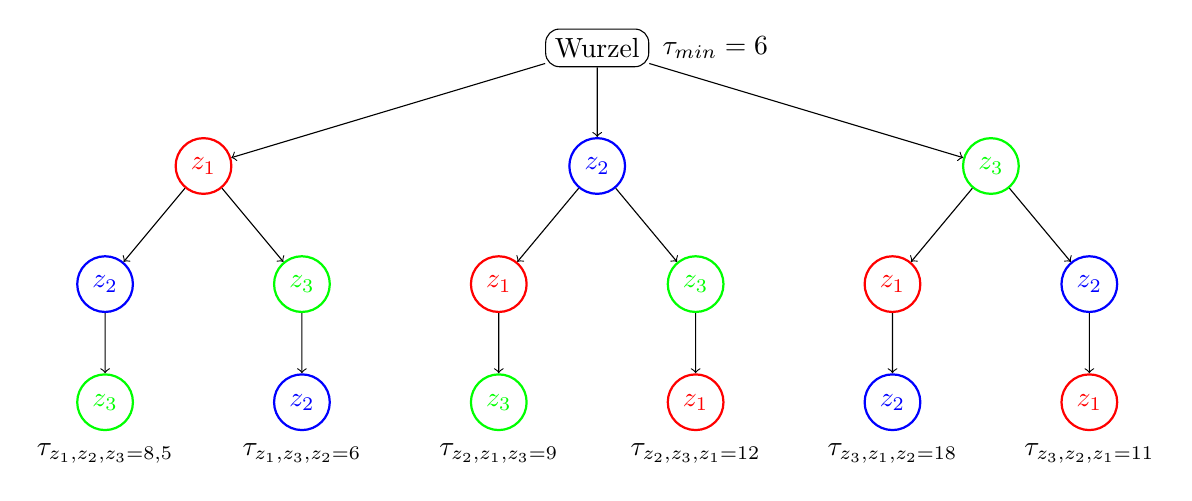
\begin{tikzpicture}[->,level/.style={sibling distance = 5cm/#1,
  level distance = 1.5cm}]
\node[rectangle, draw, rounded corners=5] (root) {Wurzel}
	child { node[red]{$z_1$}
		child { node[blue]{$z_2$}
			child { node[green](1){$z_3$} }
		}
		child { node[green]{$z_3$}
			child { node[blue](2){$z_2$} }
		}
	}
	child { node[blue]{$z_2$}
		child { node[red]{$z_1$}
			child { node[green](3){$z_3$} }
		}
		child { node[green]{$z_3$}
			child { node[red](4){$z_1$} }
		}
	}
	child { node[green]{$z_3$}
		child { node[red]{$z_1$}
			child { node[blue](5){$z_2$} }
		}
		child { node[blue]{$z_2$}
			child { node[red](6){$z_1$} }
		}
	};	
\node[above of=root, yshift=-1cm, xshift=1.5cm] {$\tau_{min} = 6$};
\node[below of=1, yshift=0.35cm] {$\tau_{z_1,z_2,z_3 = 8,5}$};
\node[below of=2, yshift=0.35cm] {$\tau_{z_1,z_3,z_2 = 6}$};
\node[below of=3, yshift=0.35cm] {$\tau_{z_2,z_1,z_3 = 9}$};
\node[below of=4, yshift=0.35cm] {$\tau_{z_2,z_3,z_1 = 12}$};
\node[below of=5, yshift=0.35cm] {$\tau_{z_3,z_1,z_2 = 18}$};
\node[below of=6, yshift=0.35cm] {$\tau_{z_3,z_2,z_1 = 11}$};
\end{tikzpicture}
\caption{Die Berechnung der jeweiligen (Teil-)Tourzeit $\tau_{i}, ~1\leq i\leq n!$ ist in diesem Fall bei nur $n!=3!=6$ Permutationen noch problemlos.}
\label{fig:BF1}
\end{figure}

\begin{figure}[htbp]
\centering
\begin{tikzpicture}[->,level/.style={sibling distance = 5cm/#1,
  level distance = 1.5cm}]
\node[rectangle, draw, rounded corners=5] (root) {Wurzel}
	child { node[red]{$z_1$}
		child { node[blue]{$z_2$}
			child { node[green]{$z_3$} }
		}
		child { node[green]{$z_3$}
			child { node[blue]{$z_2$} }
		}
	}
	child { node[blue]{$z_2$}
		child { node[red]{$z_1$}
			child { node[green]{$z_3$} }
		}
		child { node[green]{$z_3$}
			child { node[red]{$z_1$} }
		}
	}
	child { node[green](z3){$z_3$}
		child { node[gray]{$z_1$}
			child { node[gray]{$z_2$} }
		}
		child { node[gray]{$z_2$}
			child { node[gray]{$z_1$} }
		}
	};	
\node[above of=root, yshift=-1cm, xshift=1.5cm] {$\tau_{min} = 6$};
\node[below of=1, yshift=0.35cm] {$\tau_{z_1,z_2,z_3 = 8,5}$};
\node[below of=2, yshift=0.35cm] {$\tau_{z_1,z_3,z_2 = 6}$};
\node[below of=3, yshift=0.35cm] {$\tau_{z_2,z_1,z_3 = 9}$};
\node[below of=4, yshift=0.35cm] {$\tau_{z_2,z_3,z_1 = 12}$};
\node[right of=z3, xshift=0.2cm] {$\tau_{z_3} = 6.5$};
\node[red, thick, cross out, below, xshift=4.3cm, yshift=-2.1cm, rotate=50] { };
\node[red, thick, cross out, below, xshift=5.7cm, yshift=-2.1cm, rotate=-50] { };
\end{tikzpicture}
\caption{Mit der Brute-Force-Optimierung wird direkt hinter $z_3$ abgeschnitten, da an diesem Knoten bereits der Zeitpunkt $\tau_{min}$ überschritten wird.}
\label{fig:BF2}
\end{figure}

\begin{minipage}{1\linewidth}
\begin{algorithm}[H]
\begin{algorithmic}
\floatname{algorithm}{Algorithmus}
\caption{Brute-Force-Algorithmus für zwei-orthogonale Achsen beim MT-TSP}
\label{alg:BF}
\State \textbf{Input:} Targets $Z$, pursuer
\State \textbf{Output:} Targets $Z$ Targets Z in order of nondecreasing intercepting time\\

\State Sort $Z$ in order of nonincreasing absolute values of the respective velocities
\State Let $currentTargets$ be the current target order (partial permutation)
\State Let $t$ be the time-array, which represents the intercepting time for each \\
~~~~~target $z_i\in currentTargets$ 
\State $\tau_{min}\leftarrow \infty$
\State $current\leftarrow z_0$
\State $prev\leftarrow origin$, which is determined by the start position of the pursuer\\

\While {there are possible permutations remaining}
\State $current\leftarrow$ the target just intercepted
\State $prev\leftarrow$ the target previously intercepted 
\State $t[current] \leftarrow t[prev] + \pi[prev\rightarrow current]$
\If {$t[current]\geq \tau_{min}$ or at least one target of $Z\backslash currentTargets$ is located\\ ~~~~~~~~between $current$ and $prev$}
\State Step back and follow the next possible permutation-path
\Else
\If {$currentTargets$.length $\neq Z$.length}
\State Choose the next target $z_i$, $z_i\notin currentTargets$
\Else
\State $t[current]\leftarrow t[current] + \pi[current\rightarrow ursprung]$ 
\If {$t[current] < \tau_{min}$}
\State $\tau_{min}\leftarrow t[current]$
\State Step back and follow the next possible permutation-path
\EndIf 
\EndIf
\EndIf
\EndWhile
\end{algorithmic}
\end{algorithm}
\end{minipage}

\subsection{Laufzeitkomplexität Brute-Force-Ansatz}
Trotz der zuvor vorgeschlagenen Verbesserungen des Brute-Force-Algorithmus muss der worst-case betrachtet werden. Dabei gibt es in dem Permutationsbaum, welcher \emph{on-the fly} generiert wurde, an keiner Stelle im Baum eine Beschneidung nach den genannten Szenarien. Der Baum besitzt dabei $V_n = n + n\cdot (V_{n-1})$ Knoten, wodurch die Berechnung des kompletten Baums mit $\mathcal{O}(n!)$ abgeschätzt werden kann. Diese Laufzeit gilt allerdings nur für $n\leq 4$, solange die Ziele verteilt auf den Seiten \emph{Left, Right, Top} und \emph{Bottom} liegen.\\
Sobald mehr als ein Ziel auf einer Seite liegt, gibt es definitiv Beschneidungen. Für $n>4$ ist die Anzahl der Beschneidungen sehr schwer vorherzusagen. Dies hängt stark von der Eingabegröße ab. Generell konvergiert das Verhältnis von betrachteten Knoten zu $V_n$ gegen $\delta$, wobei $\delta>0$ und $n>12$ (mehr dazu im Kapitel Experimente). Eine Approximation würde dabei einen Faktor für die Laufzeit bestimmen, welcher in der Komplexität allerdings wegfällt. Somit hat der Brute-Force-Algorithmus eine Zeitkomplexität von $\mathcal{O}(n!)$.

\subsection{Korrektheit Brute-Force-Ansatz}
Mit dem Brute-Force-Algorithmus wird jede mögliche Permutation an Zielen ausprobiert. Bei der Berechnung einer Permutation werden einfach alle Ziele nacheinander abgefangen und der Zeitstempel mit der Zeit erhöht, die zum Abfangen des jeweiligen Ziels benötigt wird. Sofern eine Permutation schneller als die aktuell schnellste, wird diese übernommen und $\tau_{min}$ mit der benötigten Tourzeit überschrieben. Mit den Verbesserungen wird der Permutationsbaum beschnitten und es werden Berechnungen eingespart. Somit wird garantiert, dass die optimale Tour zurückgegeben wird.


\chapter{Experimente}

In diesem Kapitel werden die drei Algorithmen
\begin{itemize}
\item 1D-Algorithmus
\item Prioritäts-Algorithmus
\item Brute-Force-Algorithmus
\end{itemize}
mit verschiedenen Methoden getestet. Beim 1D-Algorithmus reicht es, diesen auf spezielle Eingaben zu testen. Anschließend wird beim Brute-Force-Algorithmus mit unterschiedlichen Eingabegrößen auf die Abschneidungen und die damit resultierenden Einsparungen bei der Berechnung der Permutationen getestet. Danach wird der Prioritäts-Algorithmus gegen den BF-Algorithmus laufen gelassen, um die dadurch resultierende Güte zu bestimmen. Zuletzt wird der Prioritäts-Algorithmus mit verschiedenen Kombinationen an Parametern betrachtet. 

\section{Spezielle Instanzen für den 1D-Algorithmus}

\textcolor{red}{TODO: Irgendetwas kann man doch sicherlich mit dem 1D-Fall testen. Vorschläge? Problem: In seltenen Fällen funktioniert bei einem Edge-case mein Programm nicht. Auch eine Laufzeitanalyse wäre nicht so einfach möglich, da das Programm bei manchen Instanzen eine nahezu kubische Laufzeit aufweist..}
%In diesem Kapitel sollte eine Überprüfung des 1D-Falls auf die Korrektheit der Ergebnisse  stattfinden. Die Resultate sind dafür in 


\section{Brute-Force-Algorithmus mit unterschiedlichen Eingabegrößen}

Gängige Brute-Force-Ansätze sind bei Eingabegrößen mit Zielen sehr ineffizient. Bereits bei $n=10$ ist mit $n!=3628800$ möglichen Kombinationen eine Berechnung sehr aufwendig. Mit den vorgeschlagenen Beschneidungen des Permutationsbaums soll dem Abhilfe geschaffen werden, was nun zu testen gilt. Hierfür wurde der Brute-Force-Algorithmus für verschiedene $n\in\{1,...,14\}$ getestet (siehe Tabelle \ref{tab:ExpBF}). Dabei wird die Verfolgergeschwindigkeit mit $v_{\kappa}=40$ festgesetzt. Zudem startet jedes Ziel bei einer Koordinate zwischen $-100$ und $100$ auf einer der Achsen. \\
Mit den \emph{Instanzen} werden bei einer hohen Anzahl die Ergebnisse repräsentativer. Anschließend wird für mehrere Attribute der Durchschnitt aus allen Instanzen berechnet. Die in dem Permutationsbaum \emph{betrachteten Knoten} geben an, wie viele Ziele insgesamt berechnet wurden. Somit kann mit \emph{Anteil Knoten} durch die Berechnung des Verhältnisses von den \emph{betrachteten Knoten} und $V_n$ abgewogen werden, wie viele Knoten des Baums berechnet wurde. Je niedriger dieser Wert, desto mehr wurde im Baum abgeschnitten. Mit dem $Schnitte$-Attribut kann die Anzahl an Beschneidungen im Baum bestimmt werden. Dieser Wert ist allerdings nur in Kombination mit den \emph{betrachteten Knoten} repräsentativ, da die Schnitte an jeder Stelle im Baum möglich sind\footnote{Ein Schnitt in der Nähe der Wurzel sorgt für eine starke Reduzierung an betrachteten Knoten, während ein Schnitt weit unten genau das Gegenteil bewirkt.}. Sobald eine Instanz nicht berechnet werden kann, wird dies in \emph{Fails} festgehalten.

\begin{table}[htpb]
\centering
\scalebox{0.93}{
\begin{tabular}{ccccccc} 
\uzlhline
\uzlemph{$n$} &\uzlemph{Instanzen}&\uzlemph{$\diameter$betr. Knoten} & \uzlemph{$\diameter$Anteil Knoten} & \uzlemph{$\diameter$Schnitte} & \uzlemph{$\diameter$ber. Blätter} & \uzlemph{Fails}\\ \uzlhline
1& 10000& ~~~~~~1.00& 1.000000& ~~~~~~0.00& ~~~1.00& ~0 \\
2& 10000& ~~~~~~3.75& 0.939151& ~~~~~~0.24& ~~~1.57& ~0 \\
3& 10000& ~~~~~11.75& 0.783513& ~~~~~~0.95& ~~~3.14& ~0 \\
4& 10000& ~~~~~37.81& 0.590758& ~~~~~~3.22& ~~~6.71& ~0 \\
5& 10000& ~~~~130.44& 0.401344& ~~~~~11.87& ~~15.02& ~0 \\
6& 10000& ~~~~471.76& 0.241184& ~~~~~47.23& ~~32.46& ~0 \\
7& 10000& ~~~1819.94& 0.132852& ~~~~194.96& ~~70.33& ~0 \\
8& 10000& ~~~7353.01& 0.067090& ~~~~852.13& ~150.30& ~0 \\
9& 10000& ~~31426.98& 0.031860& ~~~3833.61& ~313.76& ~0 \\
10&~1000& ~140342.54& 0.014228& ~~18169.79& ~620.86& ~0 \\
11&~1000& ~650570.40& 0.005996& ~~88862.13& 1304.56& ~0 \\
12&~~100& 3562601.51& 0.002736& ~457589.77& 3246.11& ~0 \\
13&~~100& 8184931.87& 0.000484& 1523396.29& 4303.92& 22\\
14&~~~10& 5033246.67& 0.000021& 1147070.33& 2025.67& ~7 \\ \uzlhline
\end{tabular}}
\caption{Beschneidungen im Permutationsbaum des Brute-Force-Algorithmus bei einer Eingabe von $1\leq n\leq 14$ Zielen}
\label{tab:ExpBF}
\end{table}
\noindent 
Mit der Anzahl zunehmender Eingabegröße steigt die Anzahl an betrachteten Knoten mit dem Faktor $\approx 4$ nahezu konstant an. Im Gegenzug sinkt zusätzlich der Anteil der Knoten und die Schnitte steigen. Auch die berechneten Blätter bzw. Permutationen steigen nur langsam an. Dies zeigt, dass bei ansteigender Eingabegröße, die Komplexität der Berechnung gar nicht so stark ansteigt. Bei $n=13$ werden im Schnitt gerade einmal $4303.92$ von möglichen $6227020800$ ausgerechnet. Man würde nun annehmen, dass dies auch für größere $n$ eine gute Heuristik wäre. Allerdings erkennt man schon ab $n=10$, dass die Berechnungen immer länger dauern und bei $n=14$ nur noch $10$ Berechnungen durchgeführt wurden. Dies liegt an Fällen, in denen nicht nach kurzer Zeit ein gutes $\tau_{min}$ gefunden wurde. Damit werden bei steigender Eingabegröße erheblich mehr Berechnungen durchgeführt, da der eigentliche Permutationsbaum ohne Beschneidungen eine Größe von $n!$ Permutationen besitzt.  \\
Die Ergebnisse fallen für diese Laufzeit trotzdem sehr positiv aus, da normale Brute-Force-Heuristiken bereits bei $n>10$ sehr langsam laufen und bei einer guten Vorsortierung potentiell auch Fälle mit $n=15$ durch große Abschneidungen in der Nähe der Wurzel lösbar sind. Die in diesem Fall verwendete Sortierung nach dem Betrag der Geschwindigkeit ist sehr simpel und zeigt, dass eine etwas komplexere Sortierung\footnote{Es könnten auch hier zusätzlich Prioritäten verwendet werden.} sehr wahrscheinlich schneller ein kleines $\tau_{min}$ finden kann. \\
Die Algorithmen dieser Arbeit sind jeweils in Java programmiert. Ab einer Eingabegröße von $n>12$ ereignen sich \emph{Heap-Space}-Errors. Dies liegt daran, dass zu viele Knoten betrachtet werden. Mit der Programmiersprache könnte man vermutlich $n=13$ fehlerfrei berechnen, wäre allerdings vermutlich bei $n=14$ ebenfalls limitiert. Durch die Errors ist der Datensatz mit $n=14$ nicht mehr repräsentativ, da hierbei nur drei Instanzen berechnet werden konnten. Dabei wurde bei der ersten Instanz sehr früh ein kleines $\tau_{min}$ gefunden, wodurch der Schnitt der jeweiligen Attribute sehr niedrig ist.   


\section{Güte des Prioritäts-Algorithmus}
Der Prioritäts-Algorithmus gilt mit einer Laufzeit von $\mathcal{O}(n^2)$ als sehr effizient. Da dieser keine optimalen Touren garantiert, muss nun abgeschätzt werden, ob die Ergebnisse zufriedenstellend sind. Dafür lassen wir den Algorithmus gegen den Brute-Force-Algorithmus laufen, um die Güte zu bestimmen. Der Prioritäts-Algorithmus erzeugt bei einer Instanz $I$ eine Ausgabe der Laufzeit mit $prio(I)$. Die Güte $r_I$ wird für eine Instanz mit
\begin{align*}
r_I = \dfrac{prio(I)}{opt(I)}
\end{align*} \noindent
berechnet, wobei für $opt(I)$ der Brute-Force-Algorithmus verwendet werden kann, da eine optimale Lösung garantiert wird. Da dieser bis $n=12$ einigermaßen schnell läuft, ist dies die größte Testeingabe. Für Es wird nun für jede mögliche Kombination aus den folgenden Parametern
\begin{align*}
n&\in\{8,10,12\}\\
max\{v_{i}\}\footnotemark&\in\{20,40,60\} 
\end{align*} \noindent
\footnotetext{Dies bezeichnet die Maximalgeschwindigkeit eines jeden Ziels $z_i\in Z$}
betrachtet und mit bis zu $10000$ Instanzen getestet\footnote{Die Laufzeit steigt mit der Eingabegröße stark an, demnach wird für $n=10$ und $n=12$ eine Instanzenanzahl von $1000$ bzw.  $100$ getestet.}. Mit den Instanzen wird jeweils die \emph{maximale} und \emph{durchschnittliche Güte} des Prioritäts-Algorithmus berechnet Zudem wird die Anzahl an \emph{optimalen Touren} und deren \emph{Anteil} an den Instanzen berechnet. Die Verfolgergeschwindigkeit $v_{\kappa}=61$ und die Startkoordinaten der Ziele zwischen $-100$ und $100$ werden als feste Parameter gewählt. Als Gewichte für die Berechnung der Priorität wird $\omega = \{87,34,31\}$. Diese Gewichte haben sich für verschiedene Instanzen bewährt und werden somit auch für dieses Experiment gewählt. Die Ergebnisse werden in Tabelle \ref{tab:ExpGüte} präsentiert.

\begin{table}[htpb]
\centering
\scalebox{1}{
\begin{tabular}{ccccccc} 
\uzlhline
\uzlemph{$n$} & \uzlemph{Instanzen}& \uzlemph{$max\{v_i\}$} & \uzlemph{$\diameter$Güte} & \uzlemph{max Güte} & \uzlemph{opt. Touren} & \uzlemph{Anteil opt.}\\ \uzlhline
~8& 10000& 20& 1.10& ~~2.59& 6313& 0.63 \\
~8& 10000& 40& 1.41& ~11.93& 3341& 0.33 \\
~8& 10000& 60& 3.53& 328.88& 1390& 0.14 \\
10& ~1000& 20& 1.14& ~~2.15& ~518& 0.52 \\
10& ~1000& 40& 1.54& ~~9.22& ~220& 0.22 \\
10& ~1000& 60& 5.32& 282.26& ~~83& 0.08 \\
12& ~~100& 20& 1.16& ~~2.31& ~~43& 0.43 \\
12& ~~100& 40& 1.56& ~~4.79& ~~12& 0.12 \\
12& ~~100& 60& 5.30& ~82.29& ~~~5& 0.05 \\ \uzlhline
\end{tabular}}
\caption{Güte des Prioritäts-Algorithmus}
\label{tab:ExpGüte}
\end{table}\noindent

Dies sind sehr überraschende Ergebnisse, da hierbei viele Erkenntnisse gewonnen werden. Zunächst fällt für $max\{v_i\}=60$ jeweils eine gravierende maximale Güte auf. Dies hängt damit zusammen, dass der Algorithmus nur aktuelle Ziele betrachtet und in diesem Schritt keine Berechnung für potentiell folgende Ziele getätigt wird. Bei der Durchführung ist aufgefallen, dass diese worst-case-Szenarien vor allem auftreten, sofern mehrere Zielen eine Geschwindigkeit von $v_i=61$ besitzen. Um dafür eine optimale Lösung zu garantieren, müssten auf die Instanz abgestimmte Gewichte $\omega$ gewählt werden. Durch diese Ausnahmefälle steigt auch die durchschnittliche Güte stark an. \\
Bei steigender Eingabegröße verringern sich der Anteil der optimalen Touren quasi konstant. Dies lässt vermuten, dass ab $n=14$ quasi keine optimalen Lösungen mehr gefunden werden. Mit dieser Überlegung wäre der Prioritäts-Algorithmus keine gute Option ab $n>10$, da kaum noch optimale Lösungen gefunden werden. Betrachtet man allerdings nun die durchschnittliche Güte, ist der Algorithmus vielleicht doch für große Eingabegrößen geeignet. Diese ist nahezu konstant für alle die jeweiligen maximalen Geschwindigkeiten der Ziele. Mit der konstanten durchschnittlichen Güte werden somit trotz sinkender Anzahl an optimalen Touren weiterhin schnelle Touren berechnet. Dies ist allerdings nur spekulativ, da ab $n>12$ mit dem Brute-Force-Algorithmus die Güte nicht mehr präzise genug ausgerechnet werden kann. Im Endeffekt steht und fällt der Algorithmus mit den gewählten Gewichten.

\section{Instanzen mit vielen Zielen für den Prioritäts-Algorithmus}
Es wird nun das Verhalten des Prioritäts-Algorithmus für Instanzen mit vielen Zielen getestet. Dabei kann keine Korrektheit mehr bewiesen werden, da der Brute-Force-Algorithmus für solche Eingabegrößen nicht geeignet ist. Die Startkoordinaten der Ziele liegen dabei zwischen $-250$ und $250$. Die Eingabegröße liegt für dieses Experiment zwischen $5$ und $100$. Die Geschwindigkeit wird in drei verschiedenen Kombinationen von Zielen und Verfolger getestet:
\begin{itemize}
\item $20-200$: langsame Ziele, schneller Verfolger
\item $40-100$: Differenz der Geschwindigkeiten verringert sich etwas
\item $60-~~~61$:~Verfolger ist nur minimal schneller
\end{itemize}\noindent
Diese Wahl der Startkoordinaten und Geschwindigkeiten wurden aus \cite{stieber2015multiple} übernommen. Bemerke, dass es sich bei den Geschwindigkeiten der Ziele im Gegenzug zu vorherigen Tests nicht um Maximalgeschwindigkeiten handelt, sondern festgesetzt sind. Da allerdings nur ein Verfolger betrachtet wird, kann $v_{\kappa}$ um einen Wert inkrementiert werden. Somit werden unendliche Tourzeiten verhindert. Auch in diesem Experiment werden die Gewichte $\omega = \{87,34,31\}$ verwendet. In Tabelle \ref{tab:ExpPrio} sind die Ergebnisse aus den verschiedenen Kombinationen präsentiert.

\begin{table}[htpb]
\centering
\scalebox{1}{
\begin{tabular}{cccc} 
\uzlhline
\uzlemph{$n$} & \uzlemph{$v_i$}& \uzlemph{$v_{\kappa}$} & \uzlemph{Tourzeit} \\ \uzlhline
~~5& 20 & 200 & ~~~~~~~~~~~~~~4.11 \\
~~5& 40 & 100 & ~~~~~~~~~~~~15.59 \\
~~5& 60 & ~61 & ~~~~~7198012 \\
~25& 20 & 200 & ~~~~~~~~~~~~12.75 \\
~25& 40 & 100 & ~~~~~~~~~~~136.28 \\
~25& 60 & ~61 & 1199646497 \\
~50& 20 & 200 & ~~~~~~~~~~~~13.46 \\
~50& 40 & 100 & ~~~~~~~~~~~149.14 \\
~50& 60 & ~61 & 1622776018 \\
~75& 20 & 200 & ~~~~~~~~~~~~17.28 \\
~75& 40 & 100 & ~~~~~~~~~~~168.81 \\
~75& 60 & ~61 & 1747321268 \\
100& 20 & 200 & ~~~~~~~~~~~~14.17 \\
100& 40 & 100 & ~~~~~~~~~~~164.75 \\
100& 60 & ~61 & 1615929568 \\
\uzlhline
\end{tabular}}
\caption{Ziele mit gleichen Geschwindigkeiten im Prioritäts-Algorithmus}
\label{tab:ExpPrio}
\end{table}\noindent

Mit den vorherigen Ergebnissen von Tabelle \ref{tab:ExpGüte} wird nun klar, dass die Änderungen der Geschwindigkeiten der Ziele beim Prioritäts-Algorithmus die Tourzeiten stark beeinflussen. Es kann nun grundsätzlich gesagt werden, dass der Algorithmus sehr effizient ist, sobald der Verfolger deutlich schneller ist, als jedes gegebene Ziel. Für sehr gute Ergebnisse sollte die Differenz der Geschwindigkeiten bei mindestens $40$ liegen. Für Instanzen mit sehr kleinen Differenzen sind die berechneten Touren meist weit entfernt von einer optimalen Lösung. 

%\chapter{Conclusion}
\chapter{Zusammenfassung und Ausblick}
\textcolor{red}{TODO: Zusammenfassung der Ergebnisse, v.a. aus Experimente} 
%-------------------Ergebnisse der Arbeit--------------------

\noindent
%----------------------Verbesserungen------------------------
Zwar wurden die Probleme bei der Modellierung als Graphen aufgezeigt, ausgeschlossen sei diese allerdings nicht. Mit dem Ansatz über das Lemma \ref{lem:2} sollte eine optimale Strategie definitiv möglich sein und eine geringere Laufzeit aufweist, als der Brute-Force-Algorithmus mit $\mathcal{O}(n!)$. Der Brute-Force-Ansatz kann zudem um einiges verbessert werden, indem der Permutationsbaum bereits bei der Generierung die einzelnen Ziele berechnet. Somit werden viele Permutationen gar nicht erst erstellt. Zwar wird damit eine deutlich bessere Laufzeit erzielt, bei worst-case-Fällen mit Eingaben von $n>14$ ist Brute-Force allerdings weiterhin untauglich.\\
%-------------------------Ausblick---------------------------
Mit dem Prioritätsansatz wurde zum Einen ein effizienter und mit dem Brute-Force-Ansatz zum Anderen ein optimaler Algorithmus für wenig Ziele vorgestellt. Als nächsten Schritt wäre ein einigermaßen effizienter, aber optimaler Algorithmus vom großen Interesse. Dies wäre ein notwendiger Schritt, um theoretische Arbeit für $k$-Achsen in MT-TSP zu leisten. Darüber hinaus ist das nächste Ziel in dieser Thematik die Betrachtung von zweidimensionalen MT-TSP und das Aufstellen von Heuristiken.
Diesen Jahres wurde für generelle Fälle eine Arbeit \cite{moraes} veröffentlicht, in der mit evolutionären Strategien versucht wird, auf eine optimale Tour in vielen Iterationen hinzuarbeiten. Dabei ist allerdings die optimale Tour von vielen verschiedenen Parametern abhängig und garantieren auch keine optimale Lösung. 



\begin{bibtex-entries}
@article{helvig,
  title={The moving-target traveling salesman problem},
  author={Helvig, Christopher S and Robins, Gabriel and Zelikovsky, Alex},
  journal={Journal of Algorithms},
  volume={49},
  number={1},
  pages={153--174},
  year={2003},
  publisher={Elsevier}
}

@article{moraes,
  title={Experimental Analysis of Heuristic Solutions for the Moving Target Traveling Salesman Problem Applied to a Moving Targets Monitoring System},
  author={de Moraes, Rodrigo S and de Freitas, Edison P},
  journal={Expert Systems with Applications},
  volume={136},
  pages={392--409},
  year={2019},
  publisher={Elsevier}
}

@inproceedings{hammar,
  title={Approximation results for kinetic variants of TSP},
  author={Hammar, Mikael and Nilsson, Bengt J},
  booktitle={International Colloquium on Automata, Languages, and Programming},
  pages={392--401},
  year={1999},
  organization={Springer}
}

@incollection{brandstadt1994kurzeste,
  title={K{\"u}rzeste Wege},
  author={Brandst{\"a}dt, Andreas},
  booktitle={Graphen und Algorithmen},
  pages={106--123},
  year={1994},
  publisher={Springer}
}

@article{kaaser2014algorithmen,
  title={Algorithmen und Datenstrukturen},
  author={Kaaser, Dominik S},
  year={2014}
}

@book{kunzi2013einfuhrungskursus,
  title={Einf{\"u}hrungskursus in die dynamische Programmierung},
  author={K{\"u}nzi, Hans Paul and Nievergelt, Erwin},
  volume={6},
  year={2013},
  publisher={Springer-Verlag}
}

@article{choubey2013moving,
  title={Moving target travelling salesman problem using genetic algorithm},
  author={Choubey, Nitin S},
  journal={International Journal of Computer Applications},
  volume={70},
  number={2},
  year={2013},
  publisher={Foundation of Computer Science}
}

@book{weicker2015evolutionare,
  title={Evolution{\"a}re algorithmen},
  author={Weicker, Karsten},
  pages={24--25},
  year={2015},
  publisher={Springer-Verlag}
}
  
@book{minx2015autonomes,
  title={Autonomes Fahren},
  author={Minx, Eckard and Dietrich, Rainer},
  year={2015},
  publisher={Piper ebooks}
}

@article{stieber2015multiple,
  title={The multiple traveling salesmen problem with moving targets},
  author={Stieber, Anke and F{\"u}genschuh, Armin and Epp, Maria and Knapp, Matthias and Rothe, Hendrik},
  journal={Optimization Letters},
  volume={9},
  number={8},
  pages={1569--1583},
  year={2015},
  publisher={Springer}
}

\end{bibtex-entries}

% If you need to have an appendix (I advise against it), insert it
% here using, first, \appendix and then \chapter and then,
% possibly, \section. 
%
\appendix
\chapter{Implementierungen}

\textcolor{red}{TODO} 


% \section{Experimental Parameters} % possibly
%
% Again, I advise against using an appendix.


\end{document}
